\section{Ethnographic study}\label{sec-reseach-execution}
We report the results of the ethnographic study chronologically. First, we describe the analysis of the RGUS's preferred literature sources and review the RGUS' specific experimental material. Later, we comment on our experiences replicating an existing experiment. Finally, we describe how we formalized the information into concept and process models using interviews, focus groups, and workshops.

\subsection{First Approximation}
In the first stages of the investigation, the researchers did not have an ethnographic methodology in mind but something less demanding, in line with existing qualitative studies, e.g., \cite{Johanssen-2019-Continuous-SE-support,Strandberg-2019-Ethical-Interviews-SE,Yang-2021-interview-study-developers,modi2023using,runeson2020challenges}. Accordingly, the researchers conducted interviews to clarify the RGUS knowledge and convert it directly into models. 

The interviews with RGUS members provided only limited public knowledge about experimentation. The experimenters believed that interviews were unnecessary because the researchers could acquire knowledge by studying the literature that the experimenters considered the standard, e.g., \cite{Wohlin-2000-Experimentation-SE}. Hence, we studied the literature, too.

However, communication became problematic when the interviews progressed into specialized areas, such as concrete families of experiments. For example, the experimenters supported their storytelling using specific experimental materials the researchers did not have. Nor did the researchers know to understand the experimenters' discussions. At this point, the need for a different research methodology --ethnography-- became apparent. Consequently, the researchers switched minds and continued at a slower pace. We carried out additional activities to understand the standard literature and experimental material. The interaction with the experimenters also changed. For example, the researchers participated first as experimental subjects and later as team members in one of the RGUS families of experiments.

\subsubsection{Analysis of the relevant literature}
The experimenters use the books by Wohlin \textit{et al.} \cite{Wohlin-2000-Experimentation-SE} and Juristo \& Moreno \cite{Juristo-2001-SE-experimentation} as primary sources for their experimentation process. They also utilize specific papers that advise how to experiment in SE, e.g., Basili \textit{et al.} \cite{Basili-1986-ESE}, and Kitchenham \textit{et al.} \cite{Kitchenham-2002-empirical-research-guidelines-SE}. Basili \textit{et al.}'s work \cite{Basili-1999-families-experiments} was also considered relevant due to the experimenters' interest in carrying out experimental replications.

We reviewed the literature in depth. We noticed that the sources do not use coherent terminology. At the outset, it seemed to the researchers that the literature describes different experimental procedures. They later verified that the different terms refer to essentially the same activities, e.g.:

\begin{itemize}
	\item Wohlin \textit{et al.} \cite{Wohlin-2000-Experimentation-SE}: "Experiment idea, Experiment scoping, Experiment planning, Experiment operation, Analysis \& interpretation, Presentation \& package, and Experiment report."
	\item Juristo \& Moreno \cite{Juristo-2001-SE-experimentation}: "Objective Definition, Design, Execution, and Analysis."
	\item Basili \textit{et al.} \cite{Basili-1986-ESE}: "Definition, Planning, Operation, and Interpretation."
	\item Kitchenham \textit{et al.} \cite{Kitchenham-2002-empirical-research-guidelines-SE}: "Experimental context, Experimental design, Conduct of the experiment and Data Collection, Analysis, Presentation of results, and Interpretation of results."
\end{itemize}

We looked for additional ESE books to verify whether terminological diversity was a widespread problem. We only found a new edition of Wohlin \textit{et al.}'s book \cite {Wohlin-2012-experimentatio-SE}, and the specialized books by Runeson \textit{et al.} \cite{Runenson-2012-case-study-SE} and Kitchenham \textit{et al.} \cite{Kitchenham-2015-Evidence-Based-SE}. As expected, these books share standard terms but use diverse terms throughout the text, contributing to the terminological diversity.

\subsubsection{Review of experimental material}\label{subsubsec-review-experimental-material}
The RGUS' experimental materials are a promising source of information since they represent the work performed during almost two decades of experimentation and reflect the tacit knowledge \cite{Polanyi-1996-tacit-k} present in the group. However, accessing the experimental materials was challenging; materials were scattered and disorganized. We needed the experimenters' help to find specific documents/data files, understand their structure and contents, and gain further access to related materials.

The experimental materials evolve. Experiments vary widely in documentary support, independently of their date. The experimental family explains the differences more significantly than the time; the materials related to different families of experiments show significant differences, e.g., digital raw data versus physical papers written with raw data or automatic tools to measure variables versus manual tools.

Concerning the experimental process, all experimental materials generally describe the activities carried out. The execution order and the relationship between experimental activities are unclear; they rely on the experimenters' tacit knowledge. Terminological diversity also affects experimental materials, especially among families of experiments.

We intended to reflect the RGUS knowledge in process and conceptual models. However, we largely failed to consolidate the terminology, so the resultant model, e.g., see this 
\href{https://zenodo.org/record/7093417#.YyjHb-zMLUI}{\ul{link}}, was relatively simple. However, this abstract preliminary model was satisfactory for continuing the ethnographic research.

\subsection{Becoming active participants}\label{replication}
The concepts acquired by the researchers were uncertain. We needed some external confirmation. We decided to apply the learn-by-doing methodology \cite{mendoza-2019-learn-by-doing-methodology} by experimenting and determining whether our understanding was correct.

\subsubsection{Experiment selection}
Instead of designing an experiment from scratch, the researchers replicated an experiment previously conducted by the RGUS. The replication has been published elsewhere.

Conducting a replication of the experimenters' previous work attracted their attention and guaranteed collaboration. Furthermore, the replication would allow us to recreate the design, execution, analysis, and reporting of an experiment that, until then, we only knew due to the examination of the written materials. Finally, the replication would help us better understand the experimenters' motivations and decisions.

\subsubsection{Replication planning}
Various problems hinder replication \cite{Gallardo-2012-CG-PL-SE,Vegas-2006-communication-researchers,Miller-2005-replicating-SE-experiments,Gomez-2014-understanding-replication,Demagalhaes-2015-replications-SE,Carver-2010-guidelines-replication-SE}, being the main one the absence of a detailed account of the experimental activities. For example, how to approach the experimental design, which experimental objects are necessary, and in which order. We requested the cooperation of the experimenters who ran the baseline experiment to schedule the experimental activities and adapt the design to the new context where the replication would be run.

\subsubsection{Conduction}
Efra\'in R. Fonseca C. performed a literal replication \cite{Gomez-2014-understanding-replication} in an external academic setting to the RGUS.

The existence of explicit experimental materials such as questionnaires, task descriptions, and programs significantly eased experiment conduction since the researchers defined all relevant aspects in advance. The measurement was the most complex and controversial aspect. Let us say that the experimental subjects return test cases, but these test cases are manually interpreted and not run. The experimenters' cooperation was again needed to complete the measurement. Even if the measurement procedure looked controversial, it made complete sense after discussion. We learned that the experimental protocols depend on the experimental task, which depends on the research area. The remaining steps, e.g., calculating measurements from raw data and formatting, did not imply any uncertainty. It was possible to reproduce the duplicate files used in the baseline experiment.

\subsubsection{Analysis and reporting}
We sought help to analyze and report the replication since we did not have statistical training. In retrospect, both the analysis and the report were simple to perform since the experimental design used (\textit{cross-over}) was associated with a well-defined analysis method \cite{Vegas-2016-crossover-designs-experiments-SE}. On the other hand, there were reporting guidelines available \cite{Carver-2010-guidelines-replication-SE}. The experimenters confirmed that the analysis and reporting of experiments generally do not imply substantial SE challenges.

The differences observed between replication and the baseline experiment confirmed our belief that, at least in the case of the RGUS, there are no clear guidelines that allow literal, external, and independent replication \cite{Gomez-2014-understanding-replication} of the original experiment, irrespective of the existence of incidents in the replication's execution. As a corollary, the original experimenters' presence was necessary to compare the baseline experiment results and replication.

\subsubsection{Assessment}
The replication was, in retrospect, the key to clarifying the RGUS' experimental process. The replication exercise increased the researchers' knowledge and enabled the verification of previous findings, e.g., the RGUS terminology. We made some discoveries, e.g., the specificity of experimental protocols and, notably, the confirmation of extensive tacit knowledge.

\subsection{Modeling the RGUS' knowledge}\label{subsec-conocimiento-grupo}
After the experiment, the researchers were not sure which way to go. The investigation was successful from an operational viewpoint, except for the analysis, which required specific statistical knowledge. The researchers satisfactorily completed all other activities. The models improved somehow during the replication, e.g., see this \href{https://zenodo.org/record/7101676#.YytEquzMLUI}{\ul{link}}, and to the best of our knowledge, we did not overlook anything relevant.

However, we were not completely satisfied with the ethnographic study. We replicated \textbf{one} experiment in \textbf{one} concrete SE area. Still, nothing guaranteed that we would not need the experimenters' help in a hypothetical subsequent replication \cite{Juristo-2012-replication-SE,Gomez-2014-understanding-replication}. The presence of tacit knowledge represented a severe threat to validity.

\subsubsection{Semi-structured interviews}
We decided to organize a new series of semistructured interviews with the experimenters. The key difference with the first approximation was that we would not discuss the SE experimental process \textit{in general}. Still, we would focus on replicating \textit{specific families of experiments}. Given the experience acquired during the replication, we believed this strategy could expose the tacit experimenters' knowledge.

We created an open-ended questionnaire to motivate the experimenters to give a spontaneous but relatively ordered account of their experiences. We gave up note-taking and captured the interviews with video, including the experimenters' body language. We also collected paper sketches (e.g., see Fig.~\ref{fig-proceso-exp-boseto}) that some experimenters used to support their narrative. We analyzed videos and sketches using protocol analysis \cite{Pressley-1995-verbal-protocols,sowden2020verbal}. We created a report after each interview, e.g., see this \href{https://zenodo.org/record/7102137#.YytgDOzMLUI}{\ul{link}}.

\begin{figure}[htbp!]
	\centering
	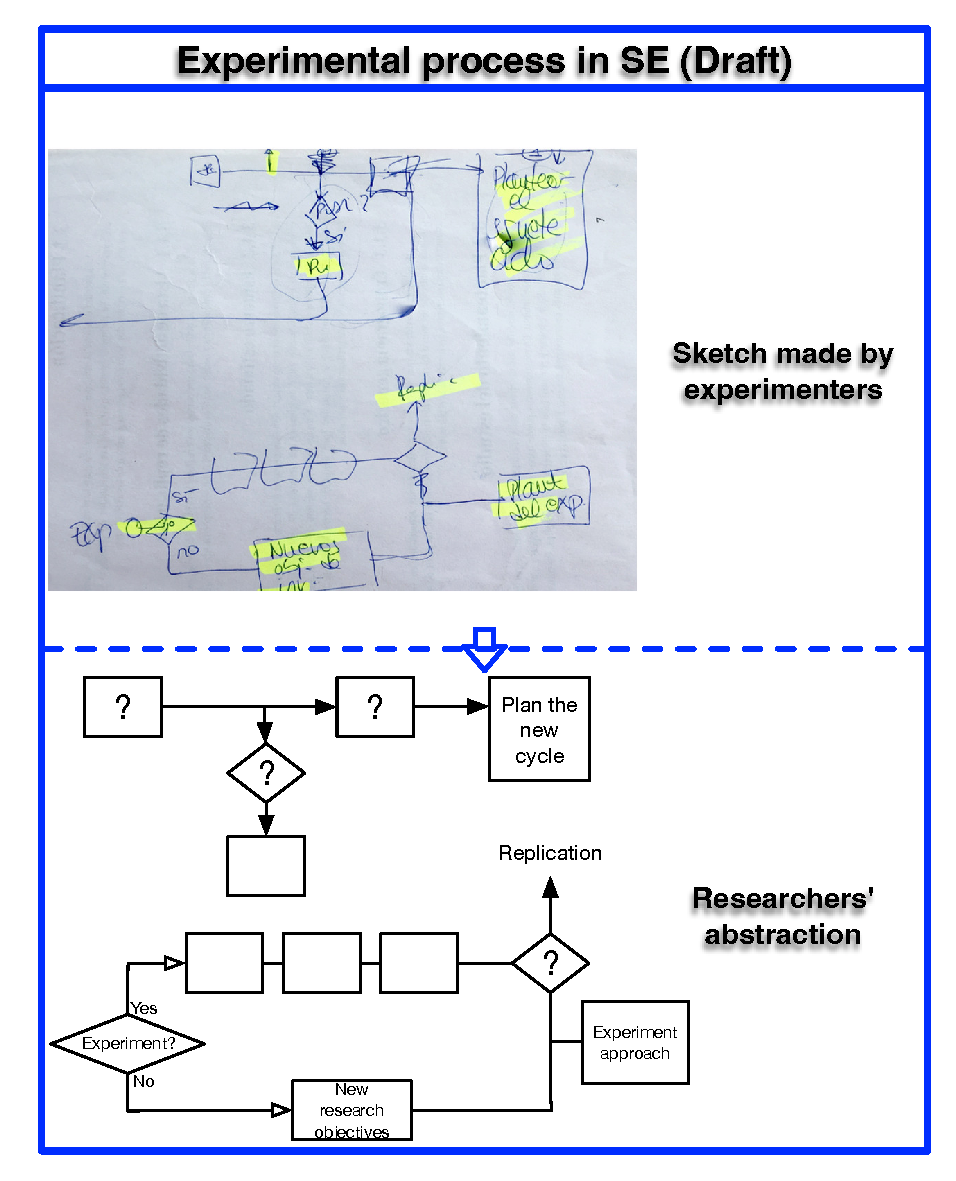
\includegraphics[width=\columnwidth]{images/Process-Approximation-Draft}
	\caption{Example of a sketch made by the experimenters. \added[id=v2]{The researchers have used drafts like this to progress in the definition of the experimental process workflow described in Section~\ref{sec-results:process-workflow}.}}
	\label{fig-proceso-exp-boseto}
	\highlight{This new figure replaces the previous Figure 2, which was included}
	\highlight{in the first version of the manuscript.}
\end{figure}


The process was smooth since each experimenter offered a coherent narrative. We conducted a total of seven interviews with six RGUS members. Each time, we refined the acquired knowledge. The reader can check the models' evolution through this \href{https://zenodo.org/record/7102213#.YytmMezMLUI}{\ul{link}}. When the progress was marginal, the interviews concluded.

\subsubsection{Preliminary models}\label{sec:preliminary-models}
We created process and concept models. We also created a workflow to represent the relations between activities that appeared during the investigation. Please note that we introduce the outstanding characteristics of the models only because the ethnographic research has not ended yet. The models and the workflow have to be validated by the experimenters. We will provide full details in Section~\ref{sec-results}.

\begin{itemize}
	\item \textit{Preliminary} experimental process model: We realized that the RGUS conducts experiments that resemble the processes we use in SE, e.g., ISO/IEC 12207 \cite{ISO-IEC-IEEE-12207}. In the end, they are all processes. Hence, we abstracted six high-level experimental processes: support, generation of pieces of knowledge, publications, synthesis, basic, and organization. Each process has several related activities. For example, the \textit{basic process} includes the activities: pre-execution (context adaptation, experiment redesign, and experiment design), execution (pre-session, in-session, and post-session), and post-execution (raw data generation, data processing, data analysis, and data interpretation) (see this \href{https://zenodo.org/record/7102301#.Yyt0GOzMLUI}{\ul{link}}).
	
\item \textit{Preliminary} workflow: It shows how the connections between experimental processes (see this \href{https://zenodo.org/record/7102360#.Yyt1a-zMLUI}{\ul{link}}). According to the experimenters, the experimental process has three main stages or paths: experimentation, replication, and synthesis. The activities performed in each step can be classified according to the experimental process model described above.

An experimenter does not usually carry out all activities, although they know how to perform them (maybe not flawlessly). In turn, different responsibilities are typically assigned to the same experimenter. We identified the following roles (the names suggest their responsibilities): (1) \textit{Research Manager}, (2) \textit{Experiment Manager}, and (3) \textit{Senior Experimenter}. These roles are responsible for (1) planning the experimental research, (2) managing the logistics, and (3) conducting the experiment in practice, respectively. The study showed overlapping responsibilities among roles, e.g., the domain and topic selection for the experiment.

	\item \textit{Preliminary} conceptual model: Preliminary results at the conceptual model level show activities similar to what the books say, indicating that it has evolved the least (see this \href{https://zenodo.org/record/7102387#.Yyt7W-zMLUI}{\ul{link}}).
\end{itemize}

\subsubsection{Double-checking using focus groups}\label{subsubsec-focus-groups}
Interviews have limitations for eliciting tacit knowledge. When the preliminary models were ready, we made a presentation to all RGUS experimenters for double-checking. 

As we said above, we organized the semistructured interviews around families of experiments. It was a fortunate mistake. The families of experiments are pretty homogeneous. The experimenters involved in the family quickly agree and provide a coherent picture of the experimental process. However, experimenters from different families disagree on many aspects, particularly the specific arrangements used in the experimental families. For instance, the experimenters never agreed on the activities related to the experimental design.

We aimed to solve the disagreements using a consensus-reaching technique, e.g., DELPHI \cite{Dalkey-1967-Delphi}. However, social pressure was not a problem. We decided to organize focus groups. The most senior experimenter led the meetings as a moderator, but only to keep the discussion on track. The researchers only observed. Each session lasted at least two hours. Before the focus group, the experimenters reviewed the concept models. We started with the concept models because they were more straightforward and smaller. The process models/workflow were later updated based on the changes to the concept model.

The focus groups prompted a substantial growth in the models' details after heated discussions that reconfirmed the existence of terminological diversity \textit{even among experimenters who carried out similar activities within the same family of experiments}. The most likely reason seems to be the training that each experimenter received. Talking about "training" in the context of the RGUS is probably incorrect since its members are self-educated, with few exceptions. The preferred SE experimental literature, e.g., \cite{Creswell-2009-Method-Approaches,montgomery-2019-Design-Analysis-Experiments}, did not drive self-education. Few of these materials existed when the experimenters started their careers. The experimenters chose the training materials according to their preferences and the experimental families in which they participated. Terminological diversity was the logical consequence.

The experimenters did not reach a consensus during the focus group exercise. The discussions with experimenters of different families exhibited a characteristic circular pattern: An experimenter triggered a change later undone by another. Substantial agreement was only possible \textit{within each family of experiments}. The progress we achieved during the replication phase of the ethnographic research (see Section~\ref {replication}) was possible due to our focus on concrete families of experiments, a fact that we completely ignored at that time.

The concept model that we obtained at this stage appears in this \href{https://zenodo.org/record/7102405#.YyuAfOzMLUI}{\ul{link}}. Notice that the agreement is apparent. 

\subsubsection{Role-focused workshops}\label{subsubsec-focus-groups-role}
We did not aim to explore SE family-specific experimental processes. Albeit enjoyable, we perceived it as future research. We tried to use the limited Ph.D. time to improve the models by switching the perspective from experimental family to \textit{experimental role}. There was no reason to think that roles could contribute to the agreement. However, we used the concept model to drive the focus groups, not the process models. Roles are connected to activities, not concepts. Activities looked more uniform than concepts. It was worth trying.

The strategy was simple. Experimenters who played the same role gathered informally and discussed the tasks associated with that role \textit{only}. Meetings were peaceful (the focus group meetings were less gentle), and the conversations were constructive. Putting aside family-specific issues, we could double-check the existence of roles (the experimenters agreed that roles make sense, even if they have never perceived their responsibilities in these terms). 

We could also break down the conceptual model into role-specific conceptual models. They represent groups of concepts the experimenters use when they play a specific role. Most experimental activities are role-specific, e.g., the senior experimenter role uses the run-kit concept exclusively. The role-specific conceptual models are available through these links: \href{https://zenodo.org/record/7102431#.YyuFvuzMLUI}{\ul{1}}, \href{https://zenodo.org/record/7102450#.YyuG2OzMLUI}{\ul{2}}, \href{https://zenodo.org/record/7102464#.YyuIkOzMLUI}{\ul{3}}.